\documentclass[11pt, letterpaper]{article}
\usepackage[utf8]{inputenc}

\makeatletter
\newcommand{\@BIBLABEL}{\@emptybiblabel}
\newcommand{\@emptybiblabel}[1]{}
\newcommand*{\permcomb}[4][0mu]{{{}^{#3}\mkern#1#2_{#4}}}
\newcommand{\perm}[1][-3mu]{\permcomb[#1]{P}}
\makeatother
\usepackage[hidelinks]{hyperref}
\usepackage{comment}
\usepackage{enumitem}
\usepackage{fullpage}
\usepackage[english]{babel}
\usepackage{graphicx}
\usepackage[colorinlistoftodos]{todonotes}
\usepackage[linesnumbered]{algorithm2e}
\usepackage{tabularx}
\usepackage{url}
\usepackage{hyperref}
\hypersetup{colorlinks=true}
\usepackage[margin=0.7in]{geometry}    % For reducing margin
\usepackage[english]{babel}
\usepackage{mathtools}
\usepackage{booktabs}
\usepackage{physics}
\usepackage{amsmath,amssymb,amsthm}
\usepackage{fullpage}
\usepackage{enumitem}
\usepackage{tcolorbox}
\usepackage{comment}
\usepackage{framed}

\newcommand{\wx}[1]{\textcolor{magenta}{\bf\small [#1 --WX]}}

\begin{document}

\title{CS 7650: Natural Language Processing (Spring 2024) \\ Problem Set 1}
\author{Instructor: Wei Xu \\ TAs: Andrew Li, Anton Lavrouk, Marcus Ma
\\Piazza: 
\url{https://piazza.com/gatech/spring2024/cs7650a}
\\Gradescope: \url{https://www.gradescope.com/courses/697909}}
\date{Due: Monday, January 29, 11:59 PM ET}
\maketitle

    \section{Logistic vs Softmax}

    \begin{enumerate}
        \item (\textbf{2 pts}) Recall the Logistic and Softmax functions
    \begin{align*}
        P_{Logistic}(y=1|\mathbf{x}) = \frac{e^{\mathbf{w}^T\mathbf{x}}}{1 + e^{\mathbf{w}^T\mathbf{x}}}
    \end{align*}
    
    \begin{align*}
        P_{Softmax}(y|\mathbf{x}) = \frac{e^{\mathbf{w}_y^T\mathbf{x}}}{\sum_{y' \in \mathcal{Y}} e^{\mathbf{w}_{y'}^T\mathbf{x}}} \\
    \end{align*}
    Given $\mathcal{Y} = \{0,1\}$, what should be the value of $\mathbf{w}$ such that $P_{Logistic}(y|\textbf{x}) = P_{Softmax}(y|\textbf{x}) \hspace{0.5em} \forall \hspace{0.5em} y \in \mathcal{Y}$? Show your work. \\ \\
    Hint: Expand the summation term and think about $\mathbf{w}$ in terms of $\mathbf{w}_0$ and $\mathbf{w}_1$. $\mathbf{w}_0$ and $\mathbf{w}_1$ are the weight vectors corresponding to the negative ($y=0$) and positive ($y=1$) classes, respectively. 
    
    \item (\textbf{2 pts}) Recall that the Softmax function is a generalization of the logistic sigmoid for multiclass classification. In practice, machine learning software such as PyTorch uses a Softmax implementation for both binary and multiclass classification. Also recall that the Softmax function produces a vector output $\mathbf{z} \in \mathbb{R}^{|\mathcal{Y}|}$ and the logistic function a single scalar value $z$, representing class probabilities. Write the equation for a decision rule to produce $\hat{y}$ from the Softmax function in the binary case (when $\mathcal{Y} = \{0,1\}$; you can break ties arbitrarily).
    Write the decision rule to produce $\hat{y}$ from the logistic function. Compare the two rules. How are they similar and/or different? (1-2 sentences).
    \end{enumerate}

\newpage
\section{Multiclass Naive Bayes with Bag of Words}

    A movie studio wants to check if their movie is being received well on social media. In particular, they want to use a Naive Bayes algorithm to automatically classify if a certain review is Positive, Neutral, or Negative. These reviews have already been passed through a feature function which returned the following key features based on the count of certain words used to describe the movie. A set of these reviews have been sampled and each were classified based on their feature vectors. The data collected so far is given in the table below:
    
    \begin{table}[h!]
    \centering
    \small
    \begin{tabular}{|l | r | r | r | r | r | r | r | r | l|}

    \hline
    S.No. & interesting & terrific & awful & strange & sad & confusing & amazing & amusing & Y \\ \hline
    1          & 1           & 0         & 0    & 1     & 1       & 0       & 0            & 0      & Positive \\
    2           & 1           & 0         & 1    & 0     & 0       & 1       & 1            & 1      & Neutral\\
    3           & 0           & 0         & 1    & 1     & 1       & 1       & 0            & 1      & Negative\\
    4           & 1           & 0         & 1    & 0     & 0       & 1       & 0            & 0      & Neutral\\
    5           & 0           & 1         & 0    & 1     & 1       & 0       & 0            & 0      & Positive\\
    6           & 0           & 1         & 0    & 0     & 0       & 0       & 1            & 0      & Neutral\\
    7           & 0           & 0         & 1    & 1     & 0       & 0       & 1            & 1      & Positive\\
    8           & 1           & 0         & 1    & 1     & 1       & 1       & 0            & 0      & Negative\\
    \hline
    \end{tabular}
    \end{table}
    
    \begin{enumerate}[label=\alph*.]
        \item (\textbf{1 pt}) What is the probability $\theta_y$ of each label $y \in$ \{Positive, Neutral, Negative\}?\\
        
        \item (\textbf{3 pts}) The parameter $\phi_{y, j}$ is the probability of a token $j$ appearing with label $y$. It is defined by the following equation, where $V$ is the size of the vocabulary set:
        $$ \phi_{y, j} = \frac{\text{count}(y, j)}{\sum^V_{j'=1}\text{count}(y, j')}$$
        
        The probability of a count of words $x$ and a label $y$ is defined as follows. Here, $\text{count}(y, j)$ represents the frequency of word $j$ appearing with label $y$ over all data points. 
        $$ \mathrm{p}(x, y; \theta, \phi) = \mathrm{p}(y; \theta) \cdot \mathrm{p}(x|y; \phi) = \mathrm{p}(y; \theta)\prod^V_{j=1} \phi^{x_j}_{y, j} $$
        
        Find the most likely label $\hat y$ for the following word counts vector $x = (1,0,0,1,1,0,1,0)$ using $\hat y = \text{argmax}_y \log \mathrm{p}(x, y; \theta; \phi)$. Show final log (base-10) probabilities for each label rounded to 3 decimals. Treat $\log(0)$ as $-\infty$. (Hint: read the above provided equations carefully; read more about \textit{binary multinomial naive Bayes} in Jurafsky \& Martin Chapter 4, as well as Hiroshi Shimodaira's note - \url{https://www.inf.ed.ac.uk/teaching/courses/inf2b/learnnotes/inf2b-learn-note07-2up.pdf}.)
        
        \item (\textbf{3 pts}) When calculating $\text{argmax}_y$, if $\phi_{y, j} = 0$ for a label-word pair, the label $y$  is no longer considered. This is an issue, especially for smaller datasets where a feature may not be present in all documents for a certain label. One approach to mitigating this high variance is to smooth the probabilities. Using add-1 smoothing, which redefines $\phi_{y, j}$, again find the most likely label $\hat y$ for the following word counts vector $x = (1,0,0,1,1,0,1,0)$ using $\hat y = \text{argmax}_y \log \mathrm{p}(x, y; \theta; \phi)$. Make sure to show final log probabilities.\\
        $$\text{add-1 smoothing: } \phi_{y, j} = \frac{1 + \text{count}(y, j)}{V + \sum^V_{j'=1}\text{count}(y, j')}$$\\
    \end{enumerate}
    
\section{Perceptron: Linear Separability and Weight Scaling}

\begin{enumerate}[label=(\alph*)]
\item (\textbf{2 pts}) Suppose we have the following data representing the XOR function:


    
Evidently, the data is not linearly separable. Therefore the perceptron algorithm will not be able to learn a classifier for XOR, based on this data.

    \begin{table}[h!]
    \centering
    \begin{tabular}{|c|c|c|}
        \hline    
         $x_1$ & $x_2$ & $f(x_1,x_2)$ \\
        \hline
        0    & 0 & -1 \\
        0    & 1 & 1 \\
        1    & 0 & 1 \\
        1    & 1 & -1 \\        
        \hline
    \end{tabular}
    \caption{XOR function data}
    \label{tab:my_label}
    \end{table}
    
However, we can add a $3^{rd}$ dimension/feature to each input such that the data becomes linearly separable. If we add $(1, 0, 0, 1)$ to the $3^{rd}$ dimension ($x_3$) of the four data points in order, will the new data be linearly separable? Assume 0 is the threshold for classification. Justify your answer.

Does the ability to add a $3^{rd}$ dimension indicate that the perceptron algorithm is capable of learning the XOR function? Why or why not?

\bigskip

\item (\textbf{2 pts}) Suppose we have a trained Perceptron with parameters $(W, b)$. If we scale $W$ by a positive constant factor $c$, will the new set of weights produce the exact same prediction for all the test data? Assume the threshold for classification is 0. Justify your answer.

\bigskip

\item (\textbf{2 pts}) With the same setting as (b), this time we translate $W$ by a positive constant factor $c$ (add $c$ to each element of $W$), will the new set of weights produce the exact same prediction for all the test data? Justify your answer.\\
\bigskip 

\end{enumerate}

\bigskip

\newpage
\section{Feedforward Neural Network}
    
    [Eisenstein Chapter 3 Problem 4] (\textbf{2 pts}) In Question 3, we tried to design a perceptron architecture in order to learn the XOR function represented by Table \ref{tab:my_label}. Now, we want you to design a feedforward neural network to compute the XOR function. This can be done in several different ways, so make sure you provide ample description of your design!\\
    
    \noindent Use a single output node and \textbf{specify} the activation function you choose for it. Also use a single hidden layer with ReLU activation function.  Describe all weights and offsets (bias terms) and ensure you design your network in accordance with Table \ref{tab:my_label}. You may draw a diagram similar to the one shown below (or just indicate the weights .\\
    
    \noindent \textit{(Hint: In class, we discussed a neural network design that solves the XOR problem using \textbf{tanh} activation functions.)}

    \begin{figure}[h]
    \centering
    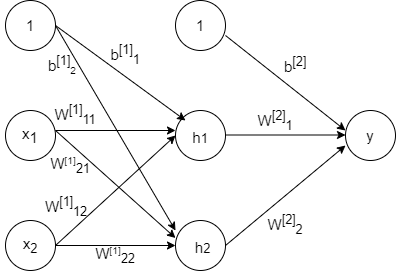
\includegraphics[width=0.4\textwidth]{images/FFNN.drawio.png}
    \caption{FFNN for XOR}
    \label{fig:my_label}
    \end{figure}
    
    \newpage
    \section{Dead Neurons}
        
    [Eisenstein Chapter 3 Problem 8] The ReLU activation function can lead to ``dead neurons'', which can never be activated on any input. Consider a feedforward neural network with a single hidden layer and ReLU nonlinearity, assuming a binary input vector, $\mathbf{x} \in f\{0,1\}^D$  and scalar output $y$:
    \begin{center}
    $z_i = \text{ReLU}(\mathbf{\theta}_i^{(x \rightarrow z)} \cdot \mathbf{x} + b_i)$ \\
    $\mathbf{y} = \mathbf{\theta}^{(z \rightarrow y)} \cdot \mathbf{z}$
    \end{center}
    
    Assume the above function is optimized to minimze a loss function (e.g., mean squared error) using stochastic gradient descent. 
    
    \begin{enumerate}
        \item (\textbf{2 pts}) Under what condition is node $z_i$ ``dead''? Your answer should be expressed in terms of the parameters $\mathbf{\theta}_i^{(x \rightarrow z)}$ and $b_i$.\\\\
        
        \item (\textbf{2 pts}) Suppose that the gradient of the loss on a given instance is $\frac{\partial l}{\partial y} = 1$. Derive gradients $\frac{\partial l}{\partial b_i}$ and $\frac{\partial l}{\partial \mathbf{\theta}_{j,i}^{(x \rightarrow z)}}$ for such an instance.\\\\
        
        \item (\textbf{2 pts}) Using your answers to the previous two parts, explain why a ``dead'' neuron can never be brought back to life during gradient-based learning. \\\\
    
    \end{enumerate}

\end{document}